\section{Wednesday for MAT4002}\index{Monday_lecture}
\subsection{Simplicial Approximation Theorem}
Aim: understand homotopy between simplicial complexes $f,g:|K|\to|L|$

\begin{definition}[Simplicial Map]
A \emph{simplicial map} between 
$K_1=(V_1,\Sigma_1)$ and $K_2=(V_2,\Sigma_2)$ is a mapping $f:K_1\to K_2$ 
such that 
\begin{enumerate}
\item
It maps vertexes to vertexes
\item
It maps simplicies to simplicies, i.e., 
\[
f(\sigma_1)\in\Sigma_2,\ \forall\sigma_1\in\Sigma_1,
\]
\end{enumerate}
\end{definition}
\begin{example}
For instance, consider the simplicial complexes defined as follows:
\begin{figure}[H]
\centering
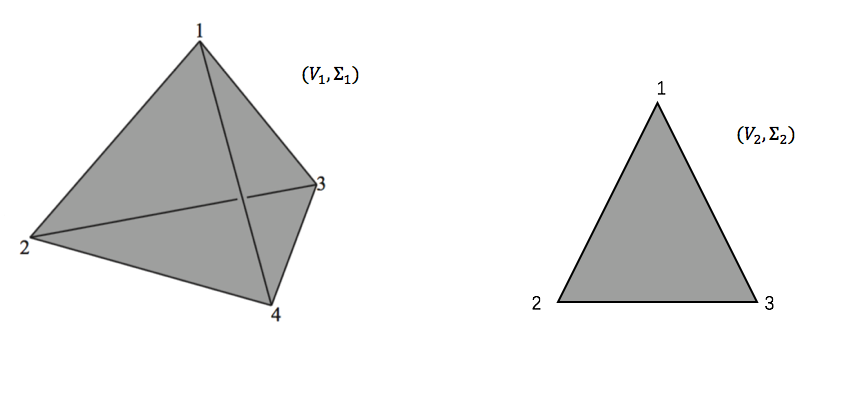
\includegraphics[width=0.6\textwidth]{week9/p_5}
\end{figure} 
In particular, $\{1,2,3,4\}\notin\Sigma_1$ and $\{1,2,3\}\in\Sigma_2$.

In this case, we can define the simplicial map as:
\[
\begin{array}{llll}
f(1)=1,&f(2)=2,&f(3)=3,&f(4)=3
\end{array}
\]
In particular, $f(\{1,2,4\})=\{1,2,3\}\in\Sigma_2$.
\end{example}

Now we want to define the simplicial map between the topological realizations. There are several observations:
\paragraph{Key Observations}
\begin{enumerate}
\item
We have seen that each $|K|\subseteq \mathbb{R}^m$ for some $m$.
In particular, $m=\# V-1$.
\item
Each point $x\in|K|$ lies uniquely on an inside of some $\Delta_\sigma,$, where $\sigma\in\Sigma$.
\item
Suppose that the vertices of $K_1$ are $V_1=\{u_1,\dots,u_n\}\subseteq\mathbb{R}^m$.
Then every $\bm x\in K_1$ can be uniquely written as
\[
\bm x=\sum_{i=1}^k\alpha_iU_{\sigma_i}
\]
with $\alpha_i>0,\sum\alpha_i=1$
and $\sigma=\{U_{\sigma_1},\dots,U_{\sigma_k}\}$ is the unqiue simplex where $x\in\text{inside}(\Delta_\sigma)$.

\begin{figure}[H]
\centering
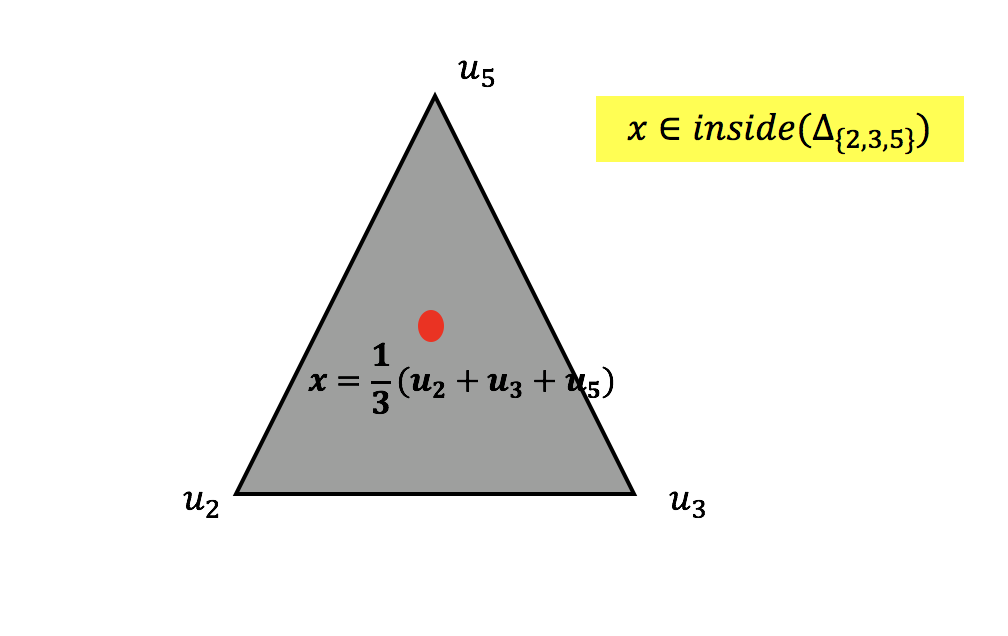
\includegraphics[width=0.6\textwidth]{week9/p_6}
\end{figure}
\item
Our simplicial map $f$ maps $V_1$ to $V_2=\{ w_1,\dots, w_p\}\subseteq\mathbb{R}^m$, so for each $i$, we have $f(\bm u_i) = \bm w_j$ for some $j\in\{1,\dots,p\}$.
\end{enumerate}

\begin{definition}[Mapping induced from Simplicial Mapping]
The simplicial map $f:K_1\to K_2$ induces a mapping $|f|:|K_1|\to|K_2|$ between the topological realizations such that
\begin{enumerate}
\item
It maps vertexes to vertexes, i.e., $|f|(v_1) = f(v_1),\forall v_1\in V(K_1)$.
\item
it is affine, i.e.,
\[
|f|\left(\sum_{i=1}^k\alpha_i v_i\right)
=
\sum_{i=1}^k\alpha_i|f|(v_i)
\]
\end{enumerate}
\end{definition}

\begin{remark}
$|f|:|K_1|\to|K_2|$ is continuous.
\end{remark}
\paragraph{Motivation}
Suppose we are given a continuous map $|g|:|K|\to|L|$, we want to {approximate} $|g|$ by $|f|$, such that $f:K\to L$ is a simplicial map.
In this case, $f$ is an easier object to study compared with $|g|$.

We hope to find a mapping $f$ such that $|f|\simeq |g|$. However, we cannot achieve this goal unless we subdivide $K$ into smaller pieces:

\begin{definition}[Subdivision]
Let $K$ be a simplicial complex.
A simplicial complex $K'$ is called a \emph{subdivision} of $K$ if
\begin{enumerate}
\item
Each simplex of $K'$ is contained in a simplex of $K$
\item
Each simplex of $K$ equals the union of finitely many simplices of $K'$
\end{enumerate}
As a result, we can form an homeomorphism $h:|K'|\to|K|$ such that for each $\sigma'\in\Sigma_{K'}$, there exists $\sigma\in\Sigma_K$ satisfying
\[
f(\Delta_{\sigma'})\in\Delta_{\sigma}
\]
\end{definition}

\begin{example}
Consider the mapping $|g|:|K|\to|L|$ given in the figure below:
\begin{figure}[H]
\centering
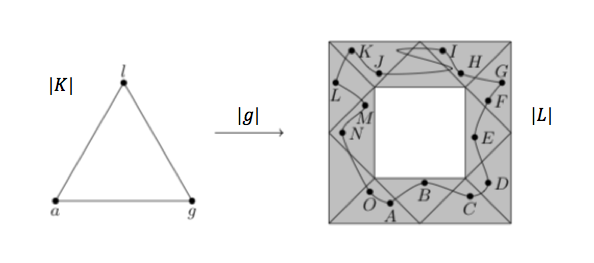
\includegraphics[width=0.55\textwidth]{week9/p_7}
\end{figure}
Here we denote $|g|(a)$ by $A$ and similarly for the other vertices.
It's clear that we can not form a homeomorphism from $|K|$ to $|L|$. One remedy is to subdivide $K$ into smaller pieces as follows: 
\begin{figure}[H]
\centering
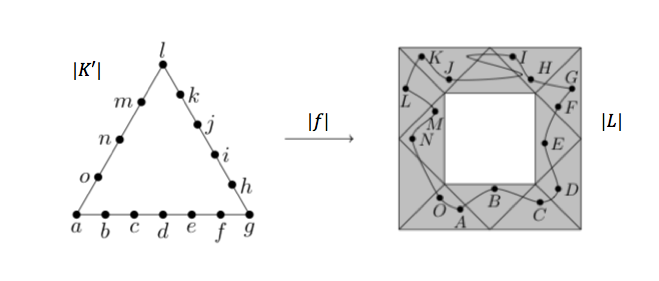
\includegraphics[width=0.55\textwidth]{week9/p_8}
\end{figure}
In this case, it is clear that $|f|:|K'|\to|L|$ is a homeomorphism.
\end{example}


\begin{example}[Barycentric Subdivision]
One typical subdivision is the Barycentric Subdivision:
\begin{figure}[H]
\centering
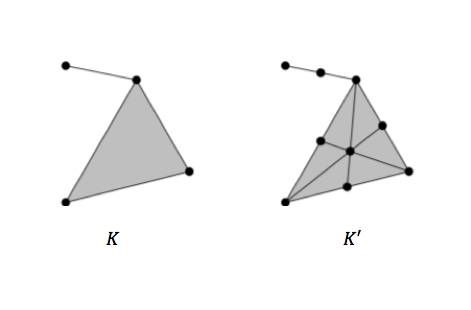
\includegraphics[width=0.6\textwidth]{week9/p_9}
\caption{Right: the subdivision of $K$}
\end{figure}
\end{example}
\begin{remark}
Suppose we have a matric on $|K|$.
By subdivision, we can consider $|K'|$ such that for any $\sigma'\in\Sigma_{K'}$, any two points in $\Delta_{\sigma'}$ has a smaller distance.
\end{remark}
The following result gives a criterion for the existence of a simplicial approximation for a mapping between topological realizations.
For this we recall the notion of star.
For a given simplicial complex $K$, define the star at a vertex $v$ by
\[
\text{star}(v)=\bigcup_{v\in\sigma}\sigma^\circ.
\]
\begin{proposition}\label{pro:9:11}
Let $f:|K|\to|L|$ be a continuous mapping.
Suppose that for each $v\in V_K$, there exists $g(v)\in V_L$ such that
\[
f(\text{st}_K(v))\subseteq \text{st}_L(g(v)),
\]
then the mapping $g:V_K\to V_K$ gives $|g|\simeq f$.

In particular, $g$ is called the \emph{simplicial approximation} to $f$.
\end{proposition}
\begin{example}
\begin{enumerate}
\item
First, we give an example of mapping $f$ such that the assumption in proposition~(\ref{pro:9:11}) is satisfied and therefore an simplicial approximation exists:
\begin{figure}[H]
\centering
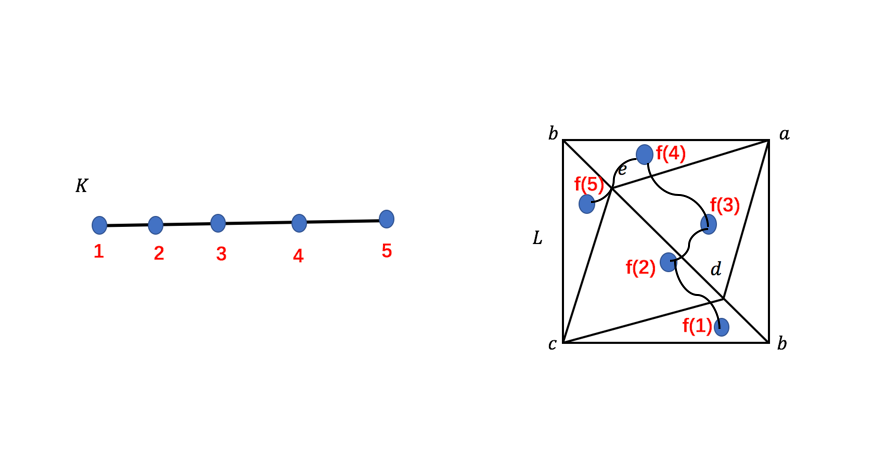
\includegraphics[width=0.8\textwidth]{week9/f_15}
\end{figure}
We could define the simplicial approximation $g$ with
\[
g(1)=b,g(2)=e,g(3)=e,g(4)=d,g(5)=d\text{ or }c
\]
\item
In the example below, the hypothesis of proposition~(\ref{pro:9:11}) is not satisfied, so we cannot apply this proposition to construct a simplicial map.
\begin{figure}[H]
\centering
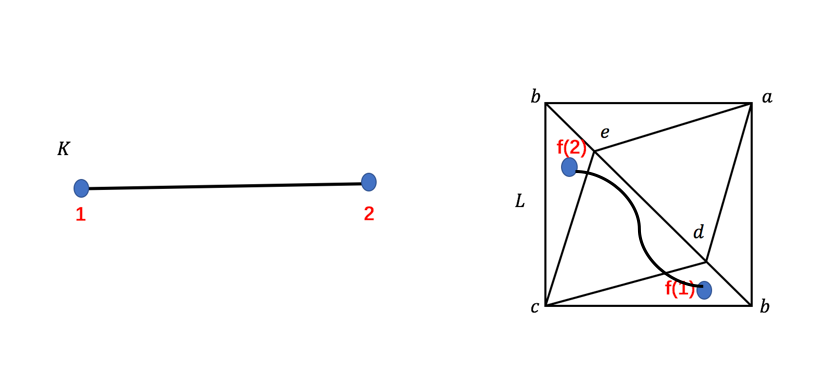
\includegraphics[width=0.8\textwidth]{week9/f_16}
\end{figure}
\end{enumerate}

\end{example}
\begin{theorem}[Simplicial Approximation]
Let $K,L$ be simplicial complexes with $V_K$ finite, and $f:|K|\to|L|$ be continuous.
Then there eixsts a subdivision $|K'|$ of $|K|$ and a simplicial map $g$ such that $|g|\simeq f$.
\end{theorem}

























